\section{Background}
\label{sec:basics}

In the following a short overview on underlying technologies is given. 

\begin{figure}
  \centering
    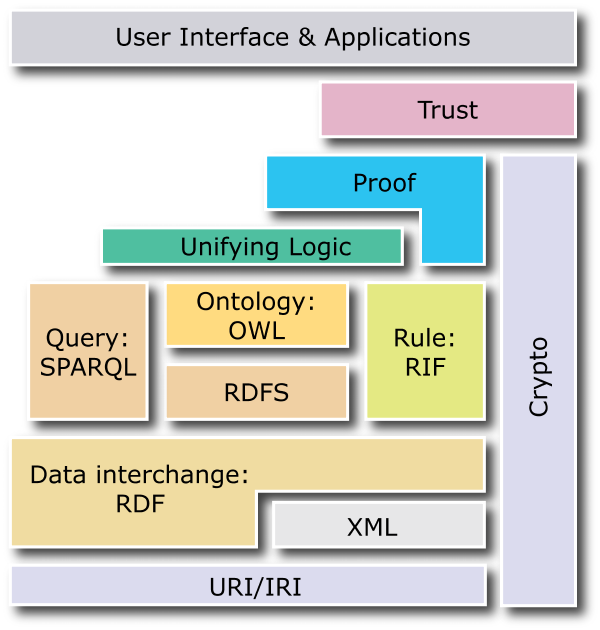
\includegraphics[width=0.5\textwidth]{layerCake.png}
  \caption{Semantic Web Technologien}
  \label{fig:layercake}
\end{figure}

\subsection{Semantic Web}

The world wide web is one the most important inventions of our time. 
It enables the global access to documents and real time communication between individuals.
This achieved by an interoperable infrastructure of independent networks, that can route any communication between two points.
From our current perspective on the last three decades, this even seems technologically simple and maintainable at a reasonable cost.
Furthermore the resulting benefits to our economy and society are beyond all expectations. A hole new industry was created and most industries are substantially influenced in their processes.
The costs of communications dropped and public and private communications alike switched mostly to the new medium.
The world wide web is enabled by a set of related technologies, which can be summarized to the following core concepts:
\begin{itemize}
\item TCP/IP addressing, transmission and routing
\item client/server communication protocols like HTTP
\item interlinked documents containing data (e.g. XML) or services (or interactive content) valuable for humans
\end{itemize}
While these technologies are well established and scale up to a huge amount of data, the users --- humans --- can barely cope with this amount of data offered. 
If one considers the WWW a information system, it only offers basic retrieval methods and most critical, it is fragmented into heterogeneous subsystems (which however can offer very good retrieval methods). 
But global interoperability is not supported on content level. Data is controlled by applications, and each application keeps it to itself\footnoteUrl{http://www.w3.org/2001/sw/}.
From a perspective of data integration, semantics are often vague or undefined. It is often unclear which entity a document refers to. Documents are only interlinked by untyped relations. These are strong limitations: if the data is too much for a human to read and machines do not have deeper insight into it, the dataset as a whole can be seen as inaccessible. Of course the way the WWW works today seems to be well suited. Programmable Webservers e.g. with PHP made the web interactive, enabling social interaction or collaborative editing. But still future development is blocked by the human-centric nature of the web. If all the knowledge humanity acquired and wrote down in e.g. Wikipedia would be also available to information systems in a structured way, even more knowledge could be inferred automatically and e.g. artificial intelligence, expert systems or search would be boosted dramatically. The key to solving this issue lies (according to \cite{berners}) in the establishment of \textit{Linked Data} (which will be explained in the next section). The use of machine readable data and annotation of text with such data is crucial for information technology to enter the next level.
So to conclude: the problem is the amount of knowledge, and the lack of formalization e.g. machine readability. Even data that is already structured often lacks a defined semantic or the semantic is not formalized. The web as we know it is a web of documents, the target is the web of data. Instead of just documents linking to each other, instances should be globally interlinked. Consider this example: A company stores costumer information about you in its relational database; facebook keeps record of your activities in their distributed database and you yourself have a blog on your own webserver. Why shouldn't all this personal information be linked\footnote{The reader may object privacy issues; but the focus of this thesis is on data integration. These two topic have to be considered separately: just because data is interoperable, it is not accessible. Even more: if you avoid redundancy, you gain control over your data. How this control can be achieved is topic to current research but already very promising. Cf. WebID}? By a global identifier for \textit{you}. Why do we have to supply contact information over and over again, although its database 101 that redundancy is bad. The answer is incompatibility on many levels. The ideal would be that all data is interoperable by design. Shortly after the invention of concepts for the WWW, Tim Berners-Lee et al. came up with the Idea of the Semantic Web: an WWW where intelligent agents can act on behalf of users, to find information or communicate. They have a shared syntax and vocabulary, use ontologies as background knowledge and thus get deeper to the intended semantic of things.
The Semantic Web (SW) is a set of complementary technologies, which are depicted in figure~\ref{fig:layercake}. It is a layered model to represent, query and manage information.\\
The effort was initiated in 2001 by Tim Berners-Lee, who defined it as 
\begin{quote}
"`an extension of the current web in which information is given well-defined
meaning, better enabling computers and people to work in cooperation"'.
\cite{berners}
\end{quote}
Dies geschieht durch verschiedene Ansätze: zunächst durch das Anreichern von (u. U. semi-struk\-tur\-iert\-en) Dokumenten durch Metainformationen schon beim Erstellungsprozess (wenn zum Beispiel ein Name in einem Dokument vorkommt, kann er in einer Art und Weise markiert werden, die allen verarbeitenden Systemen durch ein gemeinsames Vokabular als "`Personen-Markierung"' bekannt ist). Für diese Annotation wird zum Beispiel RDFa\footnoteUrl{http://www.w3.org/TR/xhtml-rdfa-primer/} genutzt. Des Weiteren wird Wissen in Form von Ontologien aufbereitet, die keine unstrukturierten Informationen enthalten, sondern lediglich \emph{wahre Aussagen} in einem formellen Format. Die Nutzung eines gemeinsamen dokumentierten Vokabulars (also die Einigung auf eine Sprache) sowie die Entwicklung offener Standards soll die Verständigung garantieren. Die Einbeziehung bereits existierender Webstandards (wie URIs oder das HTTP-Protokoll) soll eine schnelle Verbreitung ermöglichen. Dadurch soll Wissen für maschinelle Verarbeitung nutzbar gemacht werden\footnote{Allerdings wird dabei ausdrücklich nicht versucht, mithilfe künstlicher Intelligenz oder heuristischer Verfahren die Semantik für die Maschine verständlich zu machen, sondern lediglich sinnvoll repräsentierbar und damit verarbeitbar.} (vgl. \cite{hitzler}).\\
Die zentrale Technologie zur Datenrepräsentation ist RDF\footnoteUrl{http://www.w3.org/RDF/}. RDF/XML\footnoteUrl{http://www.w3.org/TR/rdf-syntax-grammar/} bzw. N3\footnoteUrl{www.w3.org/DesignIssues/Notation3} sind konkrete Kodierungen von RDF, auf welche hier nicht näher eingegangen wird. SPARQL dient als Anfragesprache für RDF-Graphen (siehe Abschnitt \ref{sec:sparql}). 

\subsection{RDF}
RDF steht für Resource Description Framework. Es ist ein Datenmodell zur Beschreibung von Web-Ressourcen (nicht nur Webseiten usw., denn jedes Ding der Welt kann über eine URI identifiziert werden), welche über eine URI\footnoteUrl{http://tools.ietf.org/html/rfc3986} identifiziert werden. Eine Ressource ist dabei eine Entität, über die Aussagen der Form \textit{"`Subjekt Prädikat Objekt"'} --- ähnlich einem natürlichsprachlichen Satz --- getroffen werden können.\\
So kodiert zum Beispiel das Tripel \\
\begin{lstlisting}[style=N3]
<http://example.com/Alice> rdf:type foaf:Person
\end{lstlisting}
die Aussage ``Alice ist eine Person''. Dabei ist Folgendes zu betrachten: Auch Subjekt, Prädikat und Objekt sind URIs, werden aber optional mit Prefixen abgekürzt (deren Definition hier ausgelassen wurde); außerdem wird das FOAF Vokabular\footnoteUrl{http://xmlns.com/foaf/0.1/} genutzt. Ein Tripel wird im Kontext der Graphentheorie interpretiert: Subjekt und Objekt sind Knoten --- das Prädikat ist der ``Typ'' der Kante.\\
\begin{figure}[h]
  \centering
    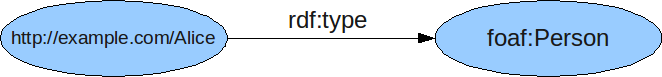
\includegraphics[width=0.5\textwidth]{triple-graph.png}
  \caption{Das Tripel als Graph}
  \label{fig:triple-graph}
\end{figure}
\\
Es entsteht (bei mehreren Tripeln) ein gerichteter Graph, der eine Ontologie repräsentiert. Graphen sind als abstraktes Konzept viel einfacher und verlässlicher zugänglich für Algorithmen als natürliche Sprache. Außerdem lassen sich implizite Informationen (zum Beispiel transitive Relationen oder geerbte Eigenschaften) ableiten oder Widersprüche finden\footnote{Access Control, Logic and Proof: \url{http://www.w3.org/2000/01/sw/#access}}.\\
Die Tatsache, dass hier kein hierarchisches Baummodell, sondern ein Graph zur Repräsentation gewählt wird, lässt sich auch damit begründen, dass Aussagen (bezüglich Beziehungen zweier Resourcen zueinander) oft nicht eindeutig einer von beiden zugeordnet werden können. Des Weiteren entspricht ein flaches Netz eher der dezentralen Struktur des Webs: Die Informationen sind verteilt und beim Zusammenführen zweier Informationsquellen stellt sich --- zumindest auf diesem Niveau --- kein Problem von Schema-Matching ein, denn das Schema ist bei allen Quellen gleichermaßen frei (vgl. \cite{hitzler}). Object-Matching soll von Beginn an vermieden werden, indem (wie oben erwähnt) ein gemeinsames Vokabular und somit überall eine eineindeutige URI für alle Objekte (Ressourcen) genutzt wird. In der Praxis besteht dieses Problem natürlich weiterhin.\\
Das Objekt eines Tripels kann in RDF auch ein Literal\footnoteUrl{http://www.w3.org/TR/rdf-concepts/#section-Graph-Literal} sein. Literale sind direkte \emph{Werte}, über die keine weiteren Aussagen getroffen werden --- also zum Beispiel Zahlen oder Zeichenketten.\\ 
Man unterscheidet zwei Arten von Literalen:
\textit{plain literals} (mit optionalem \textit{language Tag}) und \textit{typed literals}, die einen Datentyp haben, der mit einer URI angegeben wird. Im folgenden Beispiel wird das Literal mit einem selbst definierten Datentyp typisiert:

\vspace{0.2ex}

\begin{lstlisting}[style=N3]
ex:Alice foaf:birthday "22.09.1986"^^ex:germanDate
\end{lstlisting}

\subsection{Linked Data}
\textit{Linked Data} is the simplest and yet most important mechanism to retrieve RDF data: as described, entities are identified URI's. When choosing the URL's one should pick a namespace under her authority, so that she can provide \textit{some} data about that entity under that URL. As defined by W3C\footnoteUrl{http://www.w3.org/DesignIssues/LinkedData.html}, the requirements for Linked Data are as follows:

\begin{enumerate}
\item Use URIs as names for things
\item Use HTTP URIs so that people can look up those names.
\item When someone looks up an URI, provide useful information, using RDF
\item Include links to other URIs. so that they can discover more things.
\end{enumerate}
 
\begin{quotation}
The first \textit{Linked Data} principle advocates using URI references to identify, not just Web documents and digital content, but also real world objects and abstract concepts. These may include tangible things such as people, places and cars, or those that are more abstract, such as the relationship type of knowing somebody, the set of all green cars in the world, or the color green itself. This principle can be seen as extending the scope of the Web from online resources to encompass any object or concept in the world. The HTTP protocol is the Web’s universal access mechanism. In the classic Web, HTTP URIs are used to combine globally unique identification with a simple, well-understood retrieval mechanism. Thus, the second Linked Data principle advocates the use of HTTP URIs to identify objects and abstract concepts, enabling these URIs to be dereferenced (i.e., looked up) over the HTTP protocol into a description of the identified object or concept~\cite{linkeddata-book}.
\end{quotation}
The lookup of URI can even be enhanced with a mechanism called \textit{Content Negotiation}: Based on the HTTP \textit{accept} header (that is set by the application requesting), different types of formatting can be used in the response. If for example a human browses RDF data using a web browser, a HTML version of the RDF data can be generated easily. If an application requests RDF data it would set the accept header to \texttt{application/rdf+xml} and get XML, which easy to read by machines, nut not humans. The mechanism is also transparent, it happens server side at request time.  Modern RDF stores like \textit{Virtuoso} have built in support for \textit{Linked Data} with \textit{Content Negotiation}.

These four basic principles together make a fundamental difference regarding the architecture of Linked Data seen as a database. Instead of custom communication protocols, well established web standards are used. This makes it interoperable at a technical level and easy to adopt.
And it is backward compatible to very simple solutions: If one wants to publish \textit{Linked Data}, no RDF store is required at all, one could as well use a file server, with the documents available materialized.
Also \textit{Linked Data} implicitly is a \textit{basic distributed database}: Even though the query language is limited to a simple GET (for now), one can easily access data on different physical servers at no cost. Also load balancing is easy by deploying any default web proxy. Of course there if no free lunch, many topics that have been long solved on traditional relational databases, have still to be solved for RDF stores. And this little collection of advantages is not meant to compare RDF stores to relational databases, but it should show how the use of open web standards can help solving hard problems \textit{by design}. Other non-relational systems (key-value stores like Apache Cassandra or document stores like CouchDB) have shown that it is possible to make distributed databases scale and simultaneously simplify access mechanisms. RDF stores should analogously extend the expressiveness of the data model, but too be more open and designed to integrate easy.

  \begin{table}[htb]
  	\small
  	\caption{five star rating of Linked Data}
	\begin{tabular}{rp{0.7\textwidth}}
$\bigstar$ & Available on the web (whatever format) (optionally with an open licence, to be \textit{Open Data}) \\ 
$\bigstar\,\bigstar$ & Available as machine-readable structured data (e.g. excel instead of image scan of a table) \\ 
$\bigstar\,\bigstar\,\bigstar$ &  two stars plus use of a non-proprietary format (e.g. CSV instead of excel) \\ 
$\bigstar\,\bigstar\,\bigstar\,\bigstar$ & All the above plus, Use open standards from W3C (RDF and SPARQL) to identify things, so that people can point at your stuff \\ 
$\bigstar\,\bigstar\,\bigstar\,\bigstar\,\bigstar$ & All the above, plus: Link your data to other people’s data to provide context
    \end{tabular}
  \end{table}


\subsection{SPARQL}
\label{sec:sparql}
SPARQL\footnote{\url{http://www.w3.org/TR/rdf-sparql-query/} \\
bzw. \url{http://www.dajobe.org/2005/04-sparql/SPARQLreference-1.8-us.pdf}} steht für \emph{SPARQL Protocol and RDF Query Language} und ist eine Anfragesprache für RDF-Graphen sowie ein Protokoll für deren Nutzung über einen Webservice. Mit ihr können Literale, Ressourcen oder ganze Teilgraphen extrahiert werden. Sie hat sich aus anderen Sprachen, wie SquishQL\footnote{siehe \cite{squishQL}}, RDQL\footnoteUrl{http://www.w3.org/Submission/RDQL/}, RQL\footnoteUrl{http://139.91.183.30:9090/RDF/RQL/} oder SeRQL\footnote{siehe \cite{serql}} (vgl. \cite{compQL}), entwickelt und stellt nun den offiziellen Standard des W3C dar.\\
Eine kurze Übersicht\footnote{Hier werden lediglich für das weitere Verständnis zentrale Ideen erläutert --- für eine umfassende und detaillierte Beschreibung ist der Standard zu konsultieren.} über die Features der Sprache werde ich im Folgenden geben.\\
\vspace{0.1cm}\\
Es gibt 4 Typen von SPARQL Querys:
\begin{itemize}
	\item{SELECT um Daten, die auf ein angegebenes Muster passen (\emph{matchen}), zu extrahieren}
	\item{ASK um zu prüfen, \emph{ob} ein Muster im Graph existiert}
	\item{CONSTRUCT gibt einen Graph zurück, der unter Umständen durch ein Such-Muster erzeugt wurde oder explizit angegeben wird}
	\item{DESCRIBE liefert Informationen über gematchte Ressourcen (ist nicht standardisiert, abhängig von der Konfiguration der Datenbank, oft beschreibende Eigenschaften, wenn diese eingetragen wurden)}
\end{itemize}
Eine SPARQL-Anfrage (Query) lässt sich in folgende Teile aufgliedern:
\begin{itemize}
	\item{Prolog\\um Prefixe und Base-URI zu deklarieren. Relative URIs, die innerhalb des Querys vorkommen, werden auf die Base-URI bezogen. Prefixe sind Abkürzungen für häufig verwendete URIs} 
	\item{Projektionsanweisung\\ähnlich SQL: Variablen (bei SQL Spalten), welche im Ergebnis sichtbar sein sollen oder "`*"' für alle verwendeten Variablen}
	\item{Ergebnis-Modifikatoren
	\begin{itemize}
		\item{DISTINCT zur Duplikatentfernung} 
		\item{REDUCED "`kann"' Duplikate entfernen, wenn dies für die Laufzeit sinnvoll ist.}
		\item{ORDER BY sorgt für Sortierung nach einem Ausdruck (oft einer Variablen)}
		\item{LIMIT und OFFSET um einen gewisses Intervall von Lösungen auszuwählen}
	\end{itemize}
	}
	\item{GraphPattern (und Construct Pattern bei CONSTRUCT Querys)\\
	geben einen Teilgraphen an und bestehen aus Tripeln oder weiteren GraphPattern, wobei allerdings Variablen genutzt werden können --- daher der Name Pattern. Nach diesem Muster wird im Graph gesucht. Mögliche Belegungen für Variablen sind das Ergebnis.
	Es gibt folgende GraphPattern-Typen:
	\begin{itemize}
		\item{GRAPH: ein elementares Pattern, bestehend aus einer beliebigen Folge von Tripeln, weiteren GraphPattern und Filtern. Ein Tripel ist eine Aussage aus dem angefragten RDF-Graph. Zwei aufeinanderfolgende Tripel werden durch einen Punkt getrennt und bilden eine Konjenktion dieser Aussagen. Die Komponenten Subjekt, Prädikat und Objekt können durch Variablen ersetzt werden.}
		\item{OPTIONAL: ein GroupGraphPattern, das nicht notwendig ist. Das heißt: Wenn dieses Teilmuster nicht gematcht werden kann, beinflusst dies nicht das matching des gesamten Musters --- allerdings sind enthaltene Variablen dann natürlich ungebunden.} 
		\item{UNION: verknüpft mehrere GraphPattern disjunktiv. So können Alternativen ausgedrückt werden.}
	\end{itemize}
	\item{Filter sind logische Ausdrücke, die für jede mögliche Lösung\footnote{Eine Lösung ist eine Kombination von Variablen-Bindings, für die das Pattern \emph{matcht}.} evaluiert werden und (wenn sie zu \emph{false} ausgewertet werden) Ergebnisse löschen können. Für die Ausdrücke steht eine logische, numerische und relative Algebra zur Verfügung, die über eingebaute und entfernte Funktionsaufrufe erweitert wurde.
	}
	}
\end{itemize}
Ein Beispiel Query:
\begin{lstlisting}[style=sparql]
PREFIX rdf: <http://www.w3.org/1999/02/22-rdf-syntax-ns#>
PREFIX foaf: <http://xmlns.com/foaf/0.1/>
SELECT ?subj ?name
WHERE {
    ?subj rdf:type foaf:Person .
    ?subj foaf:age ?age
    OPTIONAL { ?subj foaf:name ?name }
    FILTER( ?age > 23 )
}
\end{lstlisting}
Diese Anfrage findet alle Personen, die älter als 23 sind, und, wenn möglich, deren Namen. Genauer wird folgendes ausgedrückt: Zuerst wird ein Prefix deklariert, das das RDF und FOAF Vokabular abkürzt. Im WHERE-Teil wird ein GraphPattern angegeben, mit dem die Variable \texttt{?subj} mit allen Ressourcen belegt wird, für die die Aussage gilt, dass sie vom Typ \texttt{Person} aus dem FOAF-Vokabular sind. In der siebenten Zeile wird optional der zugehörige Name an die Variable \texttt{?name} gebunden. In der sechsten und achten Zeile wird abschließend noch eine Einschränkung auf das Alter deklariert, indem zunächst der Wert an eine Variable gebunden wird und diese dann mithilfe eines Filter-Ausdrucks eingeschränkt. Bei der Auswertung dieser Anfrage wird der sogenannte Triple-Store (also eine auf RDF-Daten spezialisierte Datenbank) versuchen, dieses Muster im angefragten Graph zu finden und alle möglichen Variablen-Belegungen als Ergebnis zurückliefern --- also beispielsweise eine Tabelle oder XML mittels eines speziellen Result-Set-Formats\footnoteUrl{http://www.w3.org/TR/rdf-sparql-XMLres/}.\\
\\

\subsection{Information Extraction}

\subsection{DBpedia}

\subsection{Related Work}\label{relatedWork}
%\subsection{Comparison of Wiktionary extraction approaches}
In the last five years, the importance of \wik as a lexical-semantic resource has been examined by multiple studies.
Meyer et al. (\cite{Meyer_2010a,Meyer_2010b}) presented an impressive overview on the importance and richness of \wik. 
In \cite{Zesch_2008_jwktl} the authors presented the \emph{JWKTL} framework to access \wik dumps via a Java API.
In \cite{meyer_2011b} this JWKTL framework was used to construct an upper ontology called \emph{OntoWiktionary}.
The framework is reused within the \emph{UBY project}~\cite{Gurevych_2012}, an effort to integrate multiple lexical resources (besides \wik also \emph{WordNet}, \emph{GermaNet}, \emph{OmegaWiki}, \emph{FrameNet}, \emph{VerbNet} and \emph{Wikipedia}).
The resulting dataset is modelled according to the \emph{LMF ISO standard}\cite{iso_24613-2008}.
\cite{Moerth_2011} and \cite{Declerck-2012} discussed the use of \wik to canonicalize annotations on cultural heritage texts (namely the Thompson Motif-index). 
Zesch et. al. also showed, that \wik is suitable for calculating semantic relatedness and synonym detection; and it outperforms classic approaches~\cite{Zesch_2008,Weale_2009}. 
Furthermore, other NLP tasks such as sentiment analysis have been conducted with the help of \wik \cite{Chesley_2006}.\\
Several questions arise, when evaluating the above approaches:
Why are there not more NLP tools reusing the free \wik data?
Why are there no web mashups of the data\footnote{For example in an online dictionary from \url{http://en.wikipedia.org/wiki/List_of_online_dictionaries}}?
Why has \wik not become the central linking hub of lexical-semantic resources, yet?\\
From our point of view, the answer lies in the fact, that although the above papers presented various desirable properties and many use cases, they did not solve the underlying knowledge extraction and data integration task sufficiently in terms of coverage, precision and flexibility.
Each of the approaches presented in Table \ref{tab:sota} relies on tools to extract machine-readable data in the first place.
In our opinion these tools should  be seen independent from their respective usage and it is not our intention to comment on the scientific projects built upon them in any way here. 
We will show the state of the art and which open questions they raise. 

\begin{table}[tb]
	\begin{tabular}{l|l|l|l|l|l|l}
        \centering
        % heading
		\textbf{name} & \textbf{active} & \textbf{available} & \textbf{RDF} & \textbf{\#triples} & \textbf{ld} & \textbf{languages}\\ \hline 
        % rows
JWKTL& \tickYes & dumps & \tickNo & - & \tickNo & en, de\\ 
wikokit & \tickYes & source + dumps &  \tickYes & n/a &\tickNo & en, ru\\ 
texai& \tickNo & dumps & \tickYes & $\sim$ 2.7 million & \tickNo & en\\ 
%\footnote{See \url{http://monnetproject.deri.ie/lemonsource/} and \cite{McCrae_2012}. The Wiktionary extraction tool is just a little sub project.} 
lemon scraper & \tickYes & dumps & \tickYes &$\sim$16k per lang& \tickNo & 6\\ 
blexisma& \tickNo & source & \tickNo & - & \tickNo & en\\ 
WISIGOTH & \tickNo & dumps & \tickNo & - & \tickNo & en, fr\\ 
lexvo.org& \tickYes & dumps & \tickYes & $\sim$353k & \tickYes & en\\ 
	\end{tabular}
    \caption{Comparison of existing Wiktionary approaches (ld = linked data hosting). None of the above include any crowd-sourcing approaches for data extraction. The wikokit dump is not in RDF.}
		\label{tab:sota}
\end{table}
\textit{JWKTL} is used as data backend of \textit{OntoWiktionary} as well as  UBY\footnote{\url{http://www.ukp.tu-darmstadt.de/data/lexical-resources/uby/}, \url{http://www.ukp.tu-darmstadt.de/data/lexical-resources/uby/}} and features a modular architecture, which allows the easy addition of new extractors (for example \textit{wikokit}~\cite{wikokit} is incorporated).
The Java binaries and the data dumps in LMF are publicly available.
Among other things, the dump also contains a mapping from concepts to lexicalizations as well as properties for part of speech, definitions, synonyms and subsumption relations. 
The available languages are English, German (both natively) and Russian (through \textit{wikokit}).
According to our judgement, \textit{JWKTL} can be considered the most mature approach regarding software architecture and coverage and is the current state of the art. 
\textit{Texai}\footnoteUrl{http://sourceforge.net/projects/texai/} and \textit{Blexisma}\footnoteUrl{http://blexisma.ligforge.imag.fr/index.html} are also Java based APIs, but are not maintained anymore and were most probably made obsolete by changes to the \wik layout since 2009.
There is no documentation available regarding scope or intended granularity. 
A very fine grained extraction was conducted using WISIGOTH~\cite{sajous_2010}, but unfortunately there are no sources available and the project is unmaintained since 2010. 
Two newer approaches are the \textit{lexvo.org} service and the algorithm presented in \cite{McCrae_2012}.
The \textit{lexvo.org} service offers a linked data representation of \wik with a limited granularity, namely it does not disambiguate on sense level. 
The source code is not available and only the English \wik is parsed.
As part of the Monnet project\footnote{See \url{http://www.monnet-project.eu/}. A list of the adopted languages and dump files can be found at \url{http://monnetproject.deri.ie/lemonsource/Special:PublicLexica}}, McCrae et al.~\cite{McCrae_2012} presented a simple scraper to transform \wik to the \lemon RDF model~ \cite{lemon-eswc}.
The algorithm (like many others) makes assumptions about the used page schema and omits details about solving common difficulties (as shown in the next section). 
At the point of writing, the sources are not available, but they are expected to be published in the future. 
Although this approach appears to be the state of the art regarding RDF modelling and linking, the described algorithm will \textit{not scale to the community-driven heterogeneity} as to be defined in Section \ref{sec:problem}.
All in all, there exist various tools that implement extraction approaches at various levels of granularity or output format. 
In the next section, we will show several challenges that in our opinion are insufficiently tackled by the presented approaches. 
Note that this claim is not meant to diminish the contribution of the other approaches as they were mostly created for solving a single research challenge instead of aiming to establish \wik as a stable point of reference in computational linguistics using linked data.
\newpage
